% !TEX root = ../main.tex
\chapter{3. Requirements and Design}
\label{Requirements and Design}
In this project, a model of a rural electricity network that is disconnected from the grid is expected to be modeled. To allow the network to be scalable, the network is holonic in structure and consist of communities of prosumer "smart households" which can generate and utilise electricity depending on their demand and generation profiles. Therefore the simulator was required to have the following features:
\begin{itemize}
  \item Multiple Forms of Generation: Renewable and Non-renewable generators which can operate continuously or discontinuously
  \item Realistic Generator Models: Programmable variable generation power output to simulate wind and solar power
  \item Multiple demand centres: the simulation will be of one or more communities operating with a number of households/businesses requiring electricity
  \item Self organising by the system to allocate the available power fairly to all users
  \item Presage 2: The simulation will be programmed in Java using Presage 2.
\end{itemize}

As this was a simulation implemented in Presage 2, there were no specific requirements which must be adhered to with regards to speed, portability and performance.  

The simulation was developed using Presage 2, with the hope that a network of Decentralised Community Energy Systems can be simulated, and an algorithm for fairly allocating available generation to demand will be implemented. It is assumed that no cheating will take place.

\section*{Model Assumptions}
For the purpose of this project, all participants in the community micro-grid must be prosumers. This means all participants are expected to contribute and consume electricity. Some important assumptions will be made about how the system operates in order to simplify the implementation of both the model and the micro grid:
\begin{itemize}
	\item No losses would be incurred by the network
	\item All load on the network will be purely resistive
	\item All generation will act as negative load
	\item Only basic appliances such as phones, lights and fridges will be connected to the vast majority of households 
	\item All prosumer households will have a battery
	\item Demand requests are made automatically based on their consumption at the time without user intervention, and therefore there cheating will not take place
	\item A household will have multiple power outlets. Consumption is measured by the amount of power required to power all of these power outlets with appliances connected at full power
	\item If allocated power is below the required amount to power all of the outlets, some of the outlets will be automatically turned off by a automatic load shedding mechanism. The order which the outlets are turned off can be set by the user so the user can make sure the most important appliance is connected to the outlet that will be the last to switch off
\end{itemize}

\section*{Model Design}
To allow the Community Energy System to work as a holonic system, the micro-grid has been designed akin to the simplified model in Figure \ref{fig:SimpleModel}. The Agents in this case are reprsented by the Circles labeled A-H, with various demand/generation equipment connected to the Agents. The Agents are connected to a Virtual Agent or a Parent Agent represented by the single black dot that all Agents on the periphery are connected to in Figure \ref{fig:SimpleModel}. As the simulator is a Multi-Agent System, A Virtual Agent is employed to easily represent Group Demand and Group Generation of a small community.

\clearpage
\begin{figure}[h!]
	\centering
	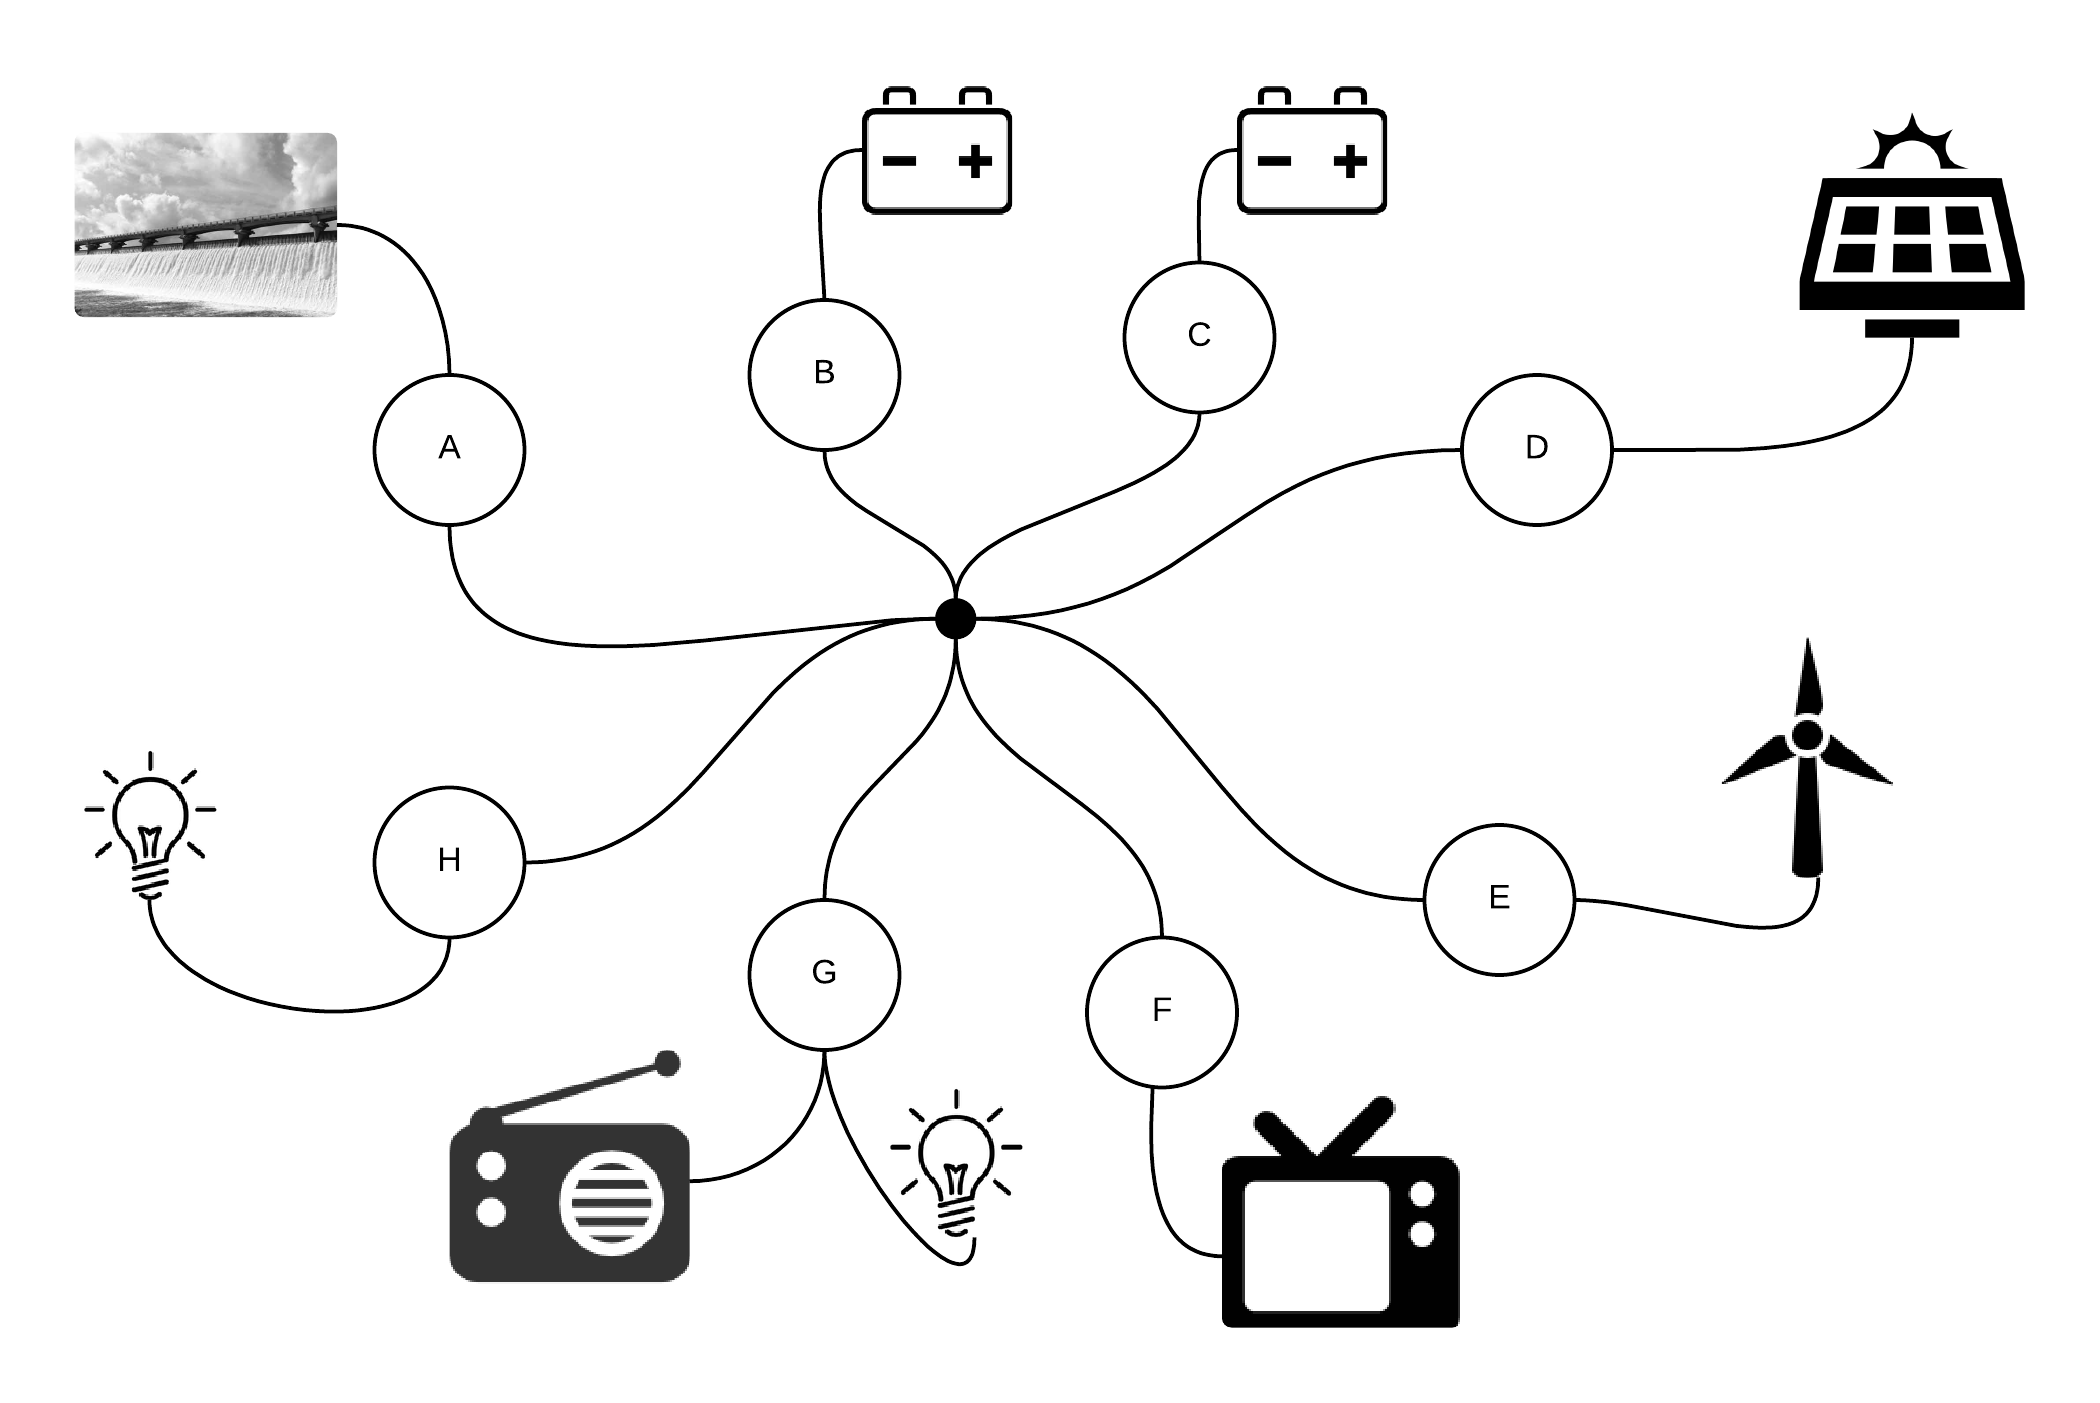
\includegraphics[scale=0.8]{Images/Model.png}
	\caption{A simplified model diagram}
	\label{fig:SimpleModel}
\end{figure}

Agents that group together are connected to a central virtual agent to allow the agents to form a community. These communities can further connected to another virtual agent to form even larger communities demonstrated in Figure \ref{fig:SimpleModel2}. 

\begin{figure}[h!]
	\centering
	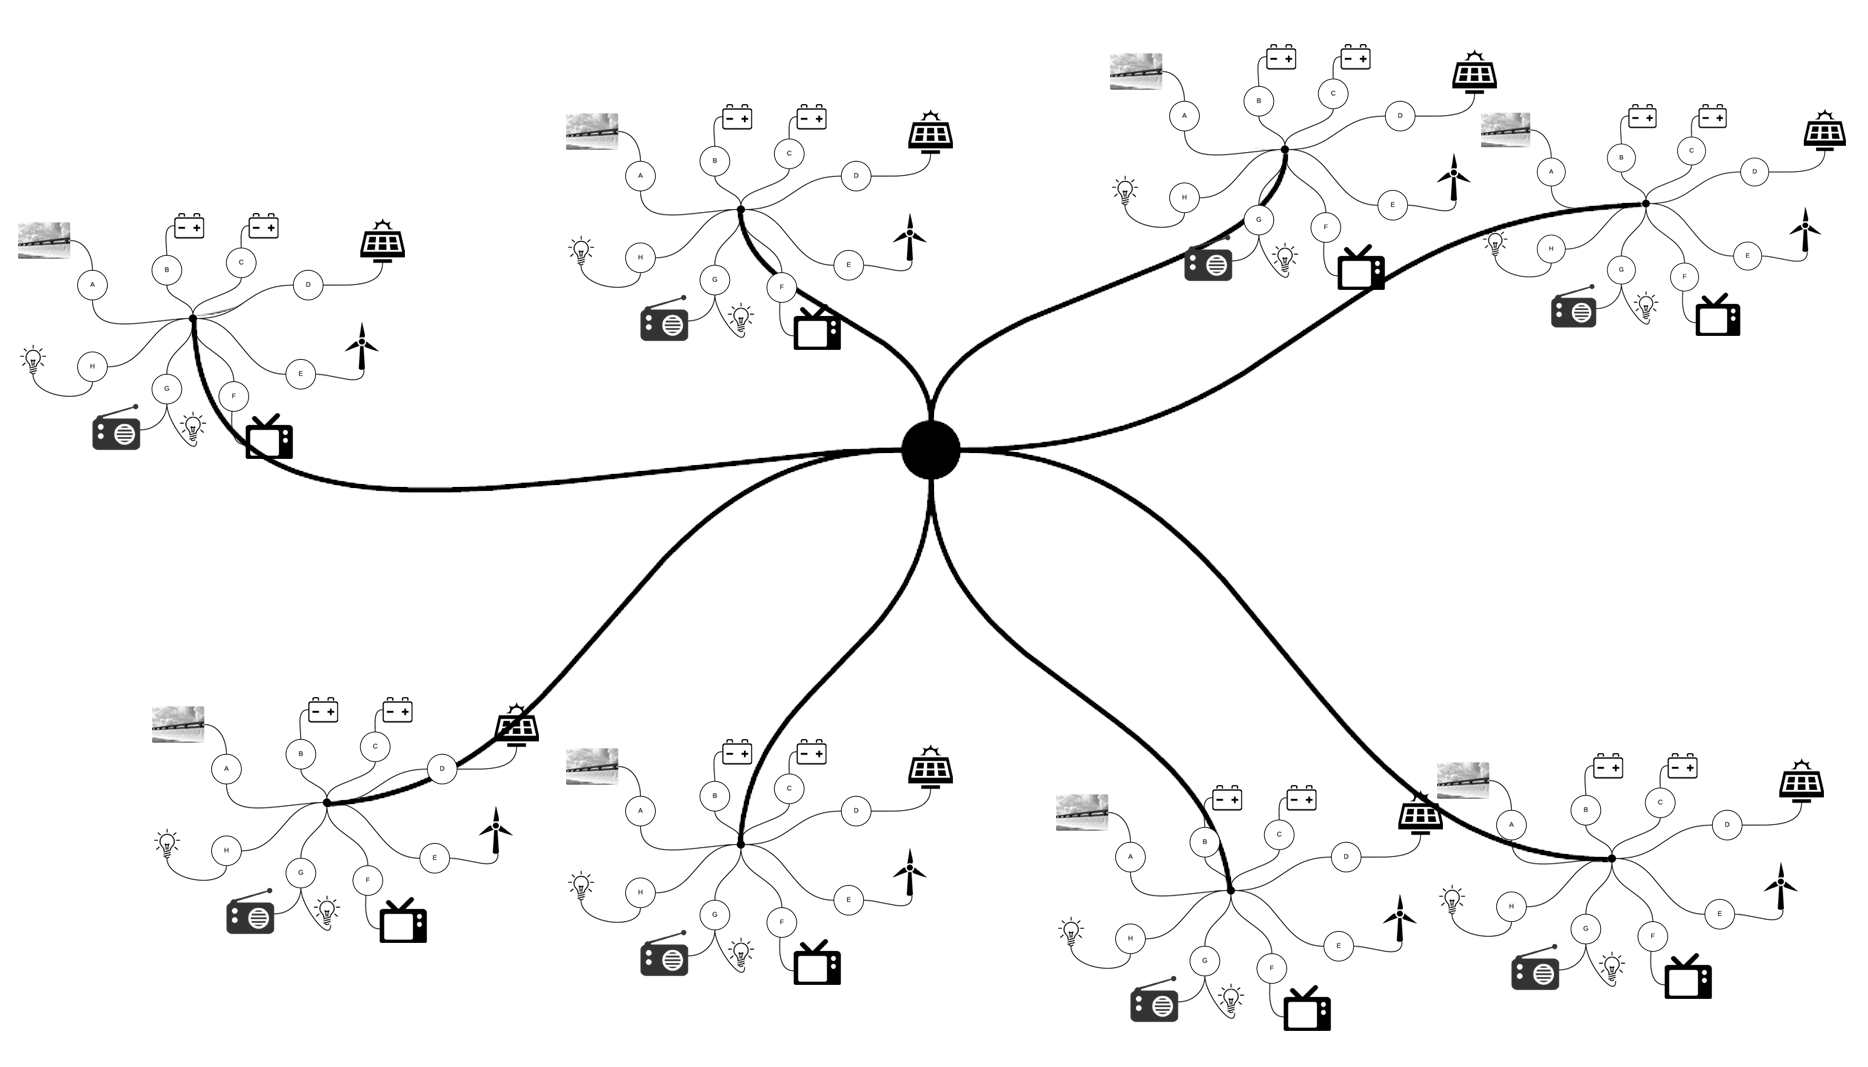
\includegraphics[scale = 0.9]{Images/Model2.png}
	\caption{A simplified network model diagram}
	\label{fig:SimpleModel2}
\end{figure}

\section*{Types of Agents}
A Multi-Agent System's main components are Agents, which are the actors which can act on the environment. Outlined below are the Agents that will be implemented as part of the simulator.
\begin{description}
\item[Virtual Agents]
represent all connected sub-communities or Agents in a community of Virtual Agents. These Agents will be responsible for enforcing quotas on connected sub-communities or Agents and collecting Generation for the Common Pool. 

\item[Prosumer Agents]
represent the most "elementary" system such as generators, households, businesses and other demand centres.
\end{description}

\section*{Agent Properties}
Agent Properties represent the information that is to be relayed to the Community or Institution that the Agent is part of.

\begin{description}
\item[Demand] - is a property which represents aggregated electricity consumption at a point of connection. Assumed demand curves will be produced from survey data of potential customers in the area for the initial testing. Should the survey data not be available for the area, a reasonable approximation will be made based a predicted usage habits of the wider local population.

It is anticipated that the final simulation will have a desired demand profile that each agent will aim to have. 

For Virtual Agents, this property represents the aggregated Demand of all connected sub-communities or Agents and will not have any associated Demand profiles.
% However, the change in demand profile due to appropriation of energy must be able to satisfy the expected behavioral habits of the local inhabitants. These habits should include restrictions such as no trading during hours of sleep for households. What the habits will be, and how this will be implemented will be determined after some additional research into the area.

\item[Generation] - is a property which will allow all agents to generate power. For Virtual Agents, this property represents the aggregated Generation of all connected sub-communities or Agents. Four types of generator properties will be implemented in this simulation model for Prosumer Agents: 

\begin{itemize}
  \item Hydro-electric - a constant source of energy based on a mixture of historical data and projections.
  \item Solar - a source of energy following the typical output profile of a solar panel connected to households.
  \item Wind - a source of energy which will be highly variable in output.
  \item Diesel - a constant source of energy.
\end{itemize}

With the power output of renewable sources of energy such as wind and solar being non-predictable in nature, one of two approach will need to be undertaken to model these sources:
\begin{itemize}
  
  \item A probabilistic generating factor is applied to the wind turbines. A constant amount of power each is assumed to be produced for a random amount of time at a random hour of the day that is to be determined. This can also happen for a random amount of times.
  
  \item An average generation power output curve is used for solar panels

\end{itemize}

A variation of both approaches are currently in use by distribution networks in the UK for assessing network congestion \cite{IPSA-web-constraint:2015}. \

\item[Storage] - Storage devices will be batteries of various types that can be connected to the network. For the purpose of this project, it will be assumed that all Prosumer Agents will have one of these to allow allocation of electricity on a hourly basis.

The Storage property should be designed have the capability to prioritise the allocation of its stored energy for certain Agents. For example, the energy output of Storage-only agents could be made to always prioritise the households they are attached to. If the battery box is communal or belongs to a centralised entity such as an e.quinox Energy Kiosk, then no priority will be attached.
\end{description}
\section*{Simulation with Presage 2}
For the initial implementation and testing, the model will only contain two levels of Aggregation designed similar to \ref{fig:SimEnv} because the micro-grid in Rugaragara Falls will be only connecting one to two communities. 

\begin{figure}[h!]
	\centering
	\includegraphics[scale = 0.41]{Figures/Environment.pdf}
	\caption{A simplified overview of the simulation structure}
	\label{fig:SimEnv}
\end{figure}

Similar to many other Multi-Agent Simulators, there can be no direct Agent-to-Agent communication. All communication must be done via the environment. As such, the environments have been designed in such a way to enable multiple levels of holonic systems that can be seen in \ref{fig:SimEnv2}. 

\begin{figure}[h!]
	\centering
	\includegraphics[scale = 0.41]{Figures/Environment3.pdf}
	\caption{A simplified overview of the simulation structure}
	\label{fig:SimEnv2}
\end{figure}

Architectually, Agents in the Simulation hold all of the information that is relevant to them. The Agents at the beginning of each allocation round submits their individual Demand and Generation request to the Virtual Agent that they are connected to. The Virtual Agents can submit their Group Demand and Group Generation Requests to other "Parent" Virtual Agents that they are connected to through the Parent Environment, and can do so recursively until the Group Demand and Generation have been sent to the Supervisor. By making the first initial allocation, the Supervisor is able to trigger a stream of allocation making by the Virtual Agents to the Virtual Agents and other Agents that are in their holonic sub-system.

\clearpage
During a round, Agents (or the houses in \ref{fig:SimEnv})are expected to publish their Demand/Generation request to the Virtual Agent that they are connected to. The Community that these parents are part of are represented by Virtual Agents. The Virtual Agent aggregates the connected Demand/Generation requests and publishes this information to the Supervisor. The Supervisor aggregates the total Demand/Generation and appropriates the electricity fairly, and curtails the generation if there is an excess.

The basic algorithm for the simulation is outlined below in Algorithm \ref{alg:basic}: \\

\begin{algorithm}[H]
	\For{each Agent} {
		request \textit{Demand} and \textit{Generation} from Virtual Agent\;
	}
	\For{each Virtual Agent} {
		request \textit{Group Demand} and \textit{Group Generation} from Supervisor Agent\;
	}
	\eIf{Group Generation >= Group Demand}{
		curtail Group Generation\;
	}{
		allocate fairly Group Demand among Virtual Agents\;
	}
	\For{each Virtual Agent} {
		allocate \textit{Group Demand} and \textit{Group Generation} allocated from Supervisor Agent\;
	}
	\caption{Basic Simulator Algorithm}
	\label{alg:basic}
\end{algorithm}

\subsection*{Time}
With the simulation being built on Presage 2, the simulation will be run in discrete time. Currently in the UK, energy is traded on a forward market at least 30 minutes ahead of consumption. In a similar fashion, the micro-grid will have the provision and allocation done on an hourly basis, one hour ahead of consumption. The Demand request will be made automatically based on their consumption at the time of allocation without user intervention. It is assumed that there is a device such a smart meter in place which can intelligently request Demand based on past user demand profiles and current electricity consumption. 

\section*{Fair Allocation of the Common Pool Resource}
With a lot of generation provided by renewable sources, there will be occurences when the aggregated Demand requests will be exceeded by the aggregated Generation requests. In circumstances such as these, electricity will need to be allocated to all users fairly. {\color{red} Rescher had observed in 1966 that a fair allocation can be found by ranking participants according to the Rescher's Canon of Distributive Justice:}

\begin{enumerate} \itemsep1pt \parskip0pt \parsep0pt
	\item Treatment as equals
	\item Treatment according to their needs
	\item Treatment according to their actual productive contribution
	\item Treatment according to their efforts and sacrifices
	\item Treatment according to a valuation of their socially-useful services
	\item Treatment according to supply and demand
	\item Treatment according to their ability, merit or achievements
\end{enumerate}


From Rescher's analysis, using each canon (criteria) alone as a basis for a claim was inadequate as it was deemed unfair. Instead, for a fair system, all canons need to be employed in conjunction with each other. In a democratic and self-organising system, the importance of each canon in the eventual allocation should be decided by the system participants. In this simulation, how the participants are ranked according to the canons are based on a similar allocation systems demonstrated in \textit{LPG'}\cite{PittSASO2012} , and are defined as below:

\begin{enumerate}
	\item \textbf{\textit{The canon of equality}} - Agents can be ranked in increasing order of their average allocations
	\item \textbf{\textit{The canon of needs}} - Assuming similar agents will have similar Demand requests, the Agent most in need is the one that has made the smallest Demand request. Therefore Agents can be ranked in increasing order of their average Demand requests.
	\item \textbf{\textit{The canon of productivity}} - Agents can be ranked in decreasing order of their economic output
	\item \textbf{\textit{The canon of effort}} - All Agents have made similar sacrifices and will gain a similar amount by being a participant of the Micro-Grid. Therefore, this canon is not represented in the simulation
	\item \textbf{\textit{The canon of social utility}} - Some Agents will provide services to the community such as providing a venue to watch a UEFA Champions League football game (something that occurs surprisingly often in rural Rwanda). Agents will be given a score of social utility based on the services they provide, and ranked in decreasing order
	\item \textbf{\textit{The canon of supply and demand}} - When allocations are required, the Agents which are most "in demand" are those Agents who contribute the most to the common pool. Therefore to encourage contribution, Agents are ranked in decreasing order of their average provision
	\item \textbf{\textit{The canon of merits and achievements}} - The merits and achievements of the Agents can't be accurately depicted in this simulation, and therefore excluded
	\item \textbf{\textit{Weighting of the canon}} - The importance placed in each of these canons when used to decide the ranking of the legitimate claims made by the participants is decided by a vote. At the end of each allocation round, participants submit a vote to decide the importance of each of the canons for the next round
	\item \textbf{\textit{Voting and multiple claims}} - To allow multiple claims to be allocated fairly, each canon and each Agent is treated as a voter in the Borda count protocol. During each allocation round, each Agent is given a number of votes by each of the canons. Under Borda count, each Agent receives a number of points corresponding to \textit{n-r+1} with n being the number of Agents being ranked, and r where the Agent placed in the ranking. For example, in a ranking of \textit{n=5} Agents, the Agent ranked first receves \textit{n-0=}5 votes, and last ranked Agent receiving \textit{n-4=}1 vote. Similarly, at the end of each allocation round, Agents rank the canons in a similar fashion to decide the points of each of the canons according to the Borda count protocol.
\end{enumerate}

%The algorithm which can allocate fairly by implementing the voting method and the canons outlined below can be found in the algorithm below

